\documentclass[11pt,preprint, authoryear]{elsarticle}

\usepackage{lmodern}
%%%% My spacing
\usepackage{setspace}
\setstretch{1.2}
\DeclareMathSizes{12}{14}{10}{10}

% Wrap around which gives all figures included the [H] command, or places it "here". This can be tedious to code in Rmarkdown.
\usepackage{float}
\let\origfigure\figure
\let\endorigfigure\endfigure
\renewenvironment{figure}[1][2] {
    \expandafter\origfigure\expandafter[H]
} {
    \endorigfigure
}

\let\origtable\table
\let\endorigtable\endtable
\renewenvironment{table}[1][2] {
    \expandafter\origtable\expandafter[H]
} {
    \endorigtable
}


\usepackage{ifxetex,ifluatex}
\usepackage{fixltx2e} % provides \textsubscript
\ifnum 0\ifxetex 1\fi\ifluatex 1\fi=0 % if pdftex
  \usepackage[T1]{fontenc}
  \usepackage[utf8]{inputenc}
\else % if luatex or xelatex
  \ifxetex
    \usepackage{mathspec}
    \usepackage{xltxtra,xunicode}
  \else
    \usepackage{fontspec}
  \fi
  \defaultfontfeatures{Mapping=tex-text,Scale=MatchLowercase}
  \newcommand{\euro}{€}
\fi

\usepackage{amssymb, amsmath, amsthm, amsfonts}

\def\bibsection{\section*{References}} %%% Make "References" appear before bibliography


\usepackage[round]{natbib}

\usepackage{longtable}
\usepackage[margin=2.3cm,bottom=2cm,top=2.5cm, includefoot]{geometry}
\usepackage{fancyhdr}
\usepackage[bottom, hang, flushmargin]{footmisc}
\usepackage{graphicx}
\numberwithin{equation}{section}
\numberwithin{figure}{section}
\numberwithin{table}{section}
\setlength{\parindent}{0cm}
\setlength{\parskip}{1.3ex plus 0.5ex minus 0.3ex}
\usepackage{textcomp}
\renewcommand{\headrulewidth}{0.2pt}
\renewcommand{\footrulewidth}{0.3pt}

\usepackage{array}
\newcolumntype{x}[1]{>{\centering\arraybackslash\hspace{0pt}}p{#1}}

%%%%  Remove the "preprint submitted to" part. Don't worry about this either, it just looks better without it:
\makeatletter
\def\ps@pprintTitle{%
  \let\@oddhead\@empty
  \let\@evenhead\@empty
  \let\@oddfoot\@empty
  \let\@evenfoot\@oddfoot
}
\makeatother

 \def\tightlist{} % This allows for subbullets!

\usepackage{hyperref}
\hypersetup{breaklinks=true,
            bookmarks=true,
            colorlinks=true,
            citecolor=blue,
            urlcolor=blue,
            linkcolor=blue,
            pdfborder={0 0 0}}


% The following packages allow huxtable to work:
\usepackage{siunitx}
\usepackage{multirow}
\usepackage{hhline}
\usepackage{calc}
\usepackage{tabularx}
\usepackage{booktabs}
\usepackage{caption}


\newenvironment{columns}[1][]{}{}

\newenvironment{column}[1]{\begin{minipage}{#1}\ignorespaces}{%
\end{minipage}
\ifhmode\unskip\fi
\aftergroup\useignorespacesandallpars}

\def\useignorespacesandallpars#1\ignorespaces\fi{%
#1\fi\ignorespacesandallpars}

\makeatletter
\def\ignorespacesandallpars{%
  \@ifnextchar\par
    {\expandafter\ignorespacesandallpars\@gobble}%
    {}%
}
\makeatother

\newenvironment{CSLReferences}[2]{%
}

\urlstyle{same}  % don't use monospace font for urls
\setlength{\parindent}{0pt}
\setlength{\parskip}{6pt plus 2pt minus 1pt}
\setlength{\emergencystretch}{3em}  % prevent overfull lines
\setcounter{secnumdepth}{5}

%%% Use protect on footnotes to avoid problems with footnotes in titles
\let\rmarkdownfootnote\footnote%
\def\footnote{\protect\rmarkdownfootnote}
\IfFileExists{upquote.sty}{\usepackage{upquote}}{}

%%% Include extra packages specified by user
\usepackage{booktabs}
\usepackage{longtable}
\usepackage{array}
\usepackage{multirow}
\usepackage{wrapfig}
\usepackage{float}
\usepackage{colortbl}
\usepackage{pdflscape}
\usepackage{tabu}
\usepackage{threeparttable}
\usepackage{threeparttablex}
\usepackage[normalem]{ulem}
\usepackage{makecell}
\usepackage{xcolor}
\usepackage{caption}
\usepackage{graphicx}
\usepackage{siunitx}
\usepackage{hhline}
\usepackage{calc}
\usepackage{tabularx}
\usepackage{adjustbox}
\usepackage{hyperref}

%%% Hard setting column skips for reports - this ensures greater consistency and control over the length settings in the document.
%% page layout
%% paragraphs
\setlength{\baselineskip}{12pt plus 0pt minus 0pt}
\setlength{\parskip}{12pt plus 0pt minus 0pt}
\setlength{\parindent}{0pt plus 0pt minus 0pt}
%% floats
\setlength{\floatsep}{12pt plus 0 pt minus 0pt}
\setlength{\textfloatsep}{20pt plus 0pt minus 0pt}
\setlength{\intextsep}{14pt plus 0pt minus 0pt}
\setlength{\dbltextfloatsep}{20pt plus 0pt minus 0pt}
\setlength{\dblfloatsep}{14pt plus 0pt minus 0pt}
%% maths
\setlength{\abovedisplayskip}{12pt plus 0pt minus 0pt}
\setlength{\belowdisplayskip}{12pt plus 0pt minus 0pt}
%% lists
\setlength{\topsep}{10pt plus 0pt minus 0pt}
\setlength{\partopsep}{3pt plus 0pt minus 0pt}
\setlength{\itemsep}{5pt plus 0pt minus 0pt}
\setlength{\labelsep}{8mm plus 0mm minus 0mm}
\setlength{\parsep}{\the\parskip}
\setlength{\listparindent}{\the\parindent}
%% verbatim
\setlength{\fboxsep}{5pt plus 0pt minus 0pt}



\begin{document}



\begin{frontmatter}  %

\title{Predicting Employee Attrition}

% Set to FALSE if wanting to remove title (for submission)




\author[Add1]{Hannah MacGinty}
\ead{21082022@sun.ac.za}





\address[Add1]{Stellenbosch University, Cape Town, South Africa}

\cortext[cor]{Corresponding author: Hannah MacGinty}

\begin{abstract}
\small{
This paper investigates employee attributes and attrition. Random
forests are used to build a model to predict employee attrition based on
key attributes, such as education, pay, gender, and age, among others.
}
\end{abstract}

\vspace{1cm}





\vspace{0.5cm}

\end{frontmatter}

\setcounter{footnote}{0}



%________________________
% Header and Footers
%%%%%%%%%%%%%%%%%%%%%%%%%%%%%%%%%
\pagestyle{fancy}
\chead{}
\rhead{}
\lfoot{}
\rfoot{\footnotesize Page \thepage}
\lhead{}
%\rfoot{\footnotesize Page \thepage } % "e.g. Page 2"
\cfoot{}

%\setlength\headheight{30pt}
%%%%%%%%%%%%%%%%%%%%%%%%%%%%%%%%%
%________________________

\headsep 35pt % So that header does not go over title




\hypertarget{introduction}{%
\section{\texorpdfstring{Introduction
\label{Introduction}}{Introduction }}\label{introduction}}

Losing employees can be costly for businesses. Predicting attrition and
its key determinants or attributes can help estimate future employee
turnover and attempt to reduce it.

\hypertarget{exploratory-data-analaysis}{%
\section*{Exploratory Data Analaysis}\label{exploratory-data-analaysis}}
\addcontentsline{toc}{section}{Exploratory Data Analaysis}

The dataset contains information on 4653 employees and whether they
attrited or not. The employee attributes available include demographic
information such as age and gender. Employees are based in one of three
major cities in India, namely Bangalore, Pune and New Delhi. The year an
employee joined a company (Joining Year), ranging from 2014 to 2018, is
also considered.

Given that earnings are generally an important determinant in whether an
employee leaves their job, their payment tier, scaled from 1, being the
highest, and 3, being the lowest, is included in the data. Additionally,
years of experience in their current field is included as well as their
highest level of education (Bachelor's, Master's, PhD). There is also
information on whether an employee kept out of projects for 1 month or
more, which could potentially indicates an employee's lack of interest
in work or plans to leave the company.

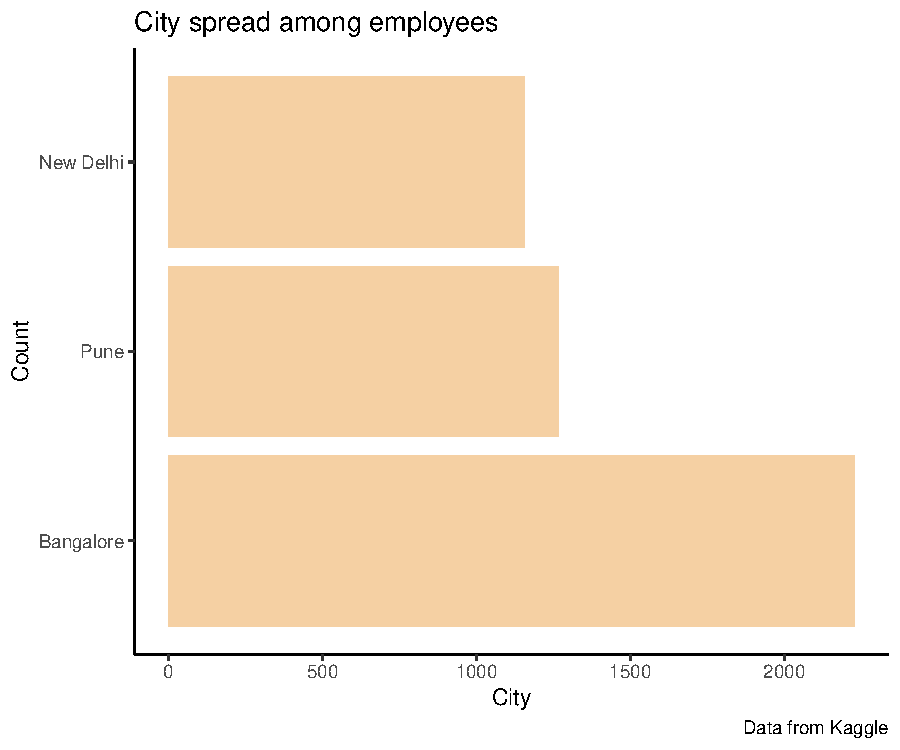
\includegraphics{Final_project_files/figure-latex/unnamed-chunk-2-1.pdf}
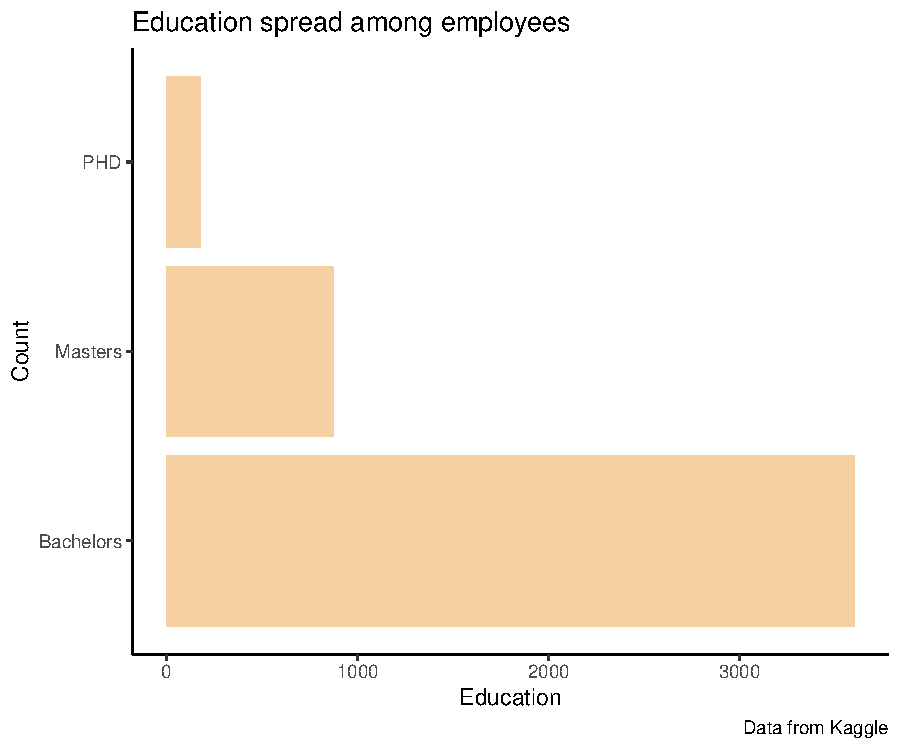
\includegraphics{Final_project_files/figure-latex/unnamed-chunk-2-2.pdf}

Spreading the data among city, most of the employees are from Bangalore.
Additionally, most employees have a Bachelors degree. Only 179 employees
have a PHD and 873 have Master's degrees. Looking at age, which ranges
between 22 and 41, the majority of employees are in their mid to late
twenties, skewing the distribution to right.

Regarding experience, very few individuals have 6 or 7 years experience
(only 16 employees in total) in their current field of work, most likely
due to the young employee base. Most commonly, individuals have 2 years
experience.

2017 saw the most employees join the company. There was a substantial
fall in employees joining in 2018. Only 367 employees joined in 2018,
compared to 1180 in 2017.

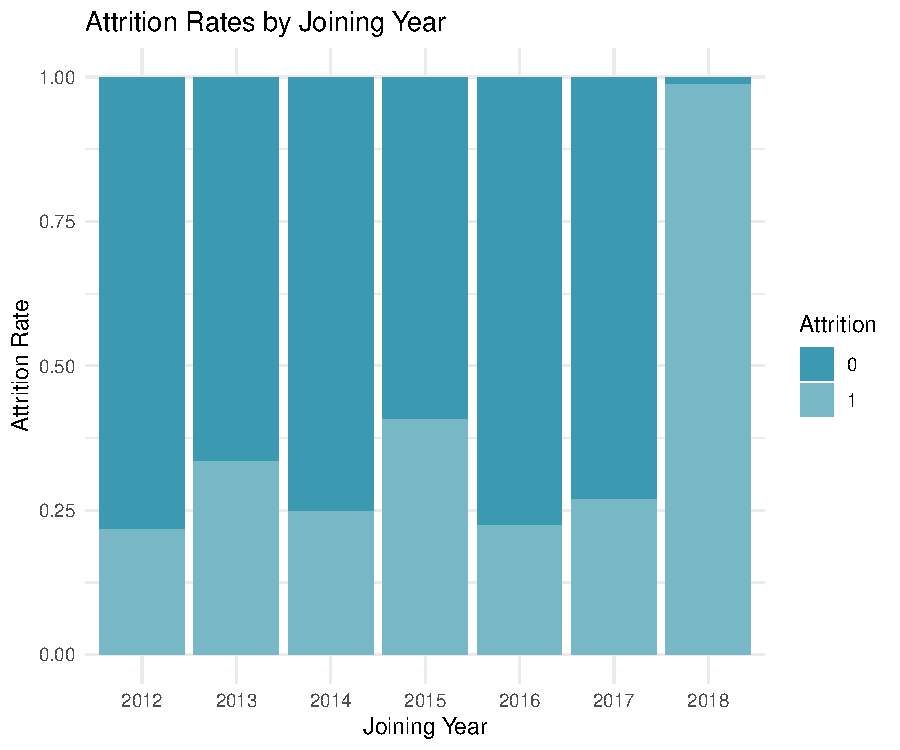
\includegraphics{Final_project_files/figure-latex/unnamed-chunk-3-1.pdf}
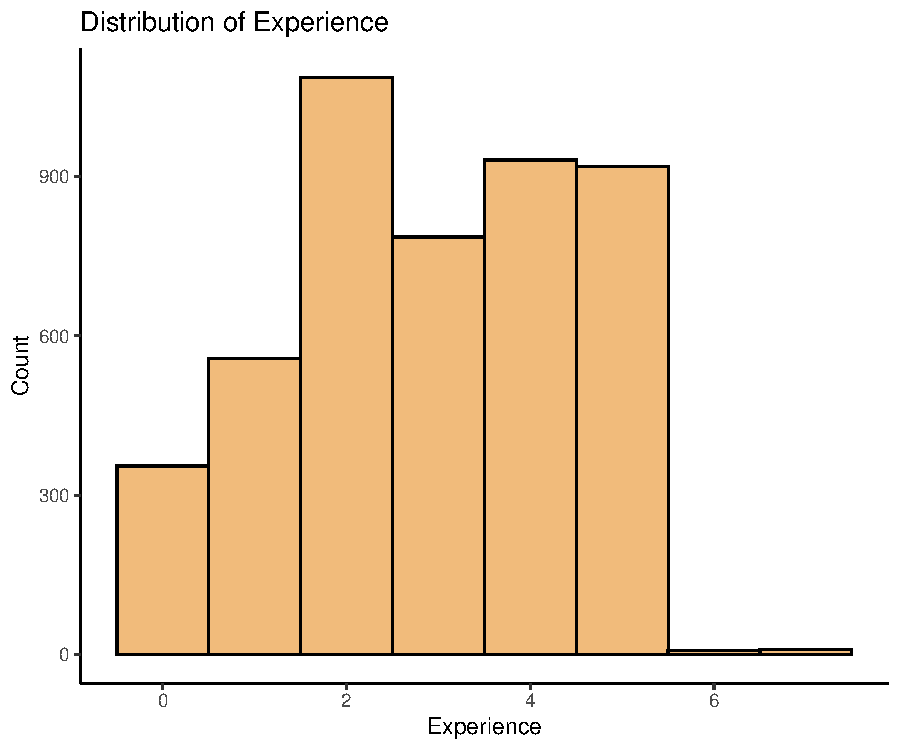
\includegraphics{Final_project_files/figure-latex/unnamed-chunk-3-2.pdf}
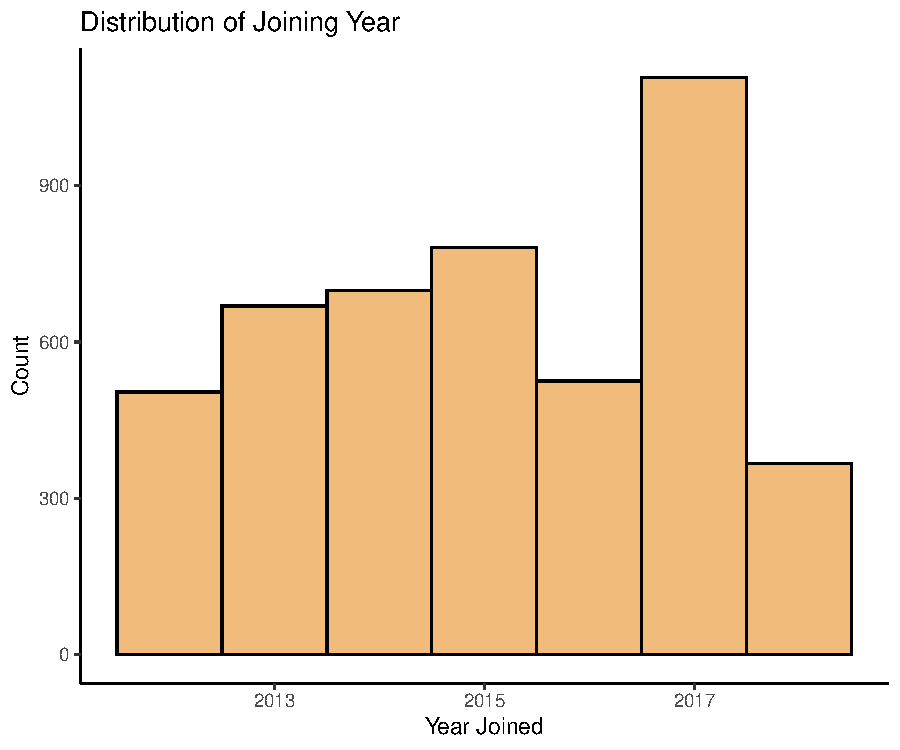
\includegraphics{Final_project_files/figure-latex/unnamed-chunk-3-3.pdf}

Attrition rates are highest among those with Master's degrees. Nearly
fifty percent of those with Master's degrees left their job. When
looking across joining year, almost all the employees that joined in
2018 resigned. It is possible that some event occurred in 2018 that
caused that cohort to leave within the next two years.

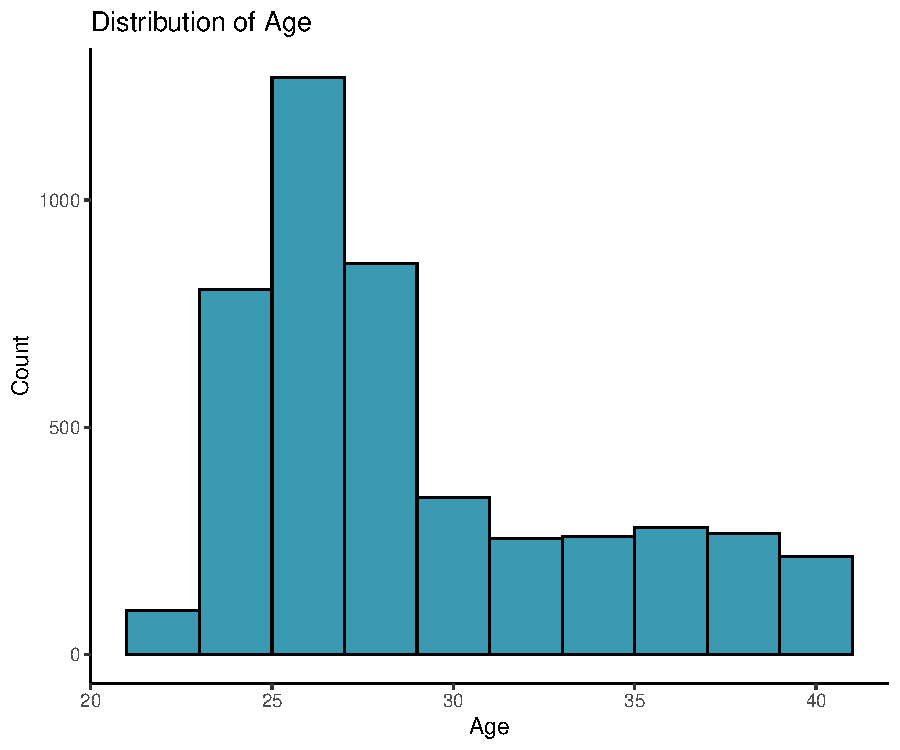
\includegraphics{Final_project_files/figure-latex/unnamed-chunk-4-1.pdf}
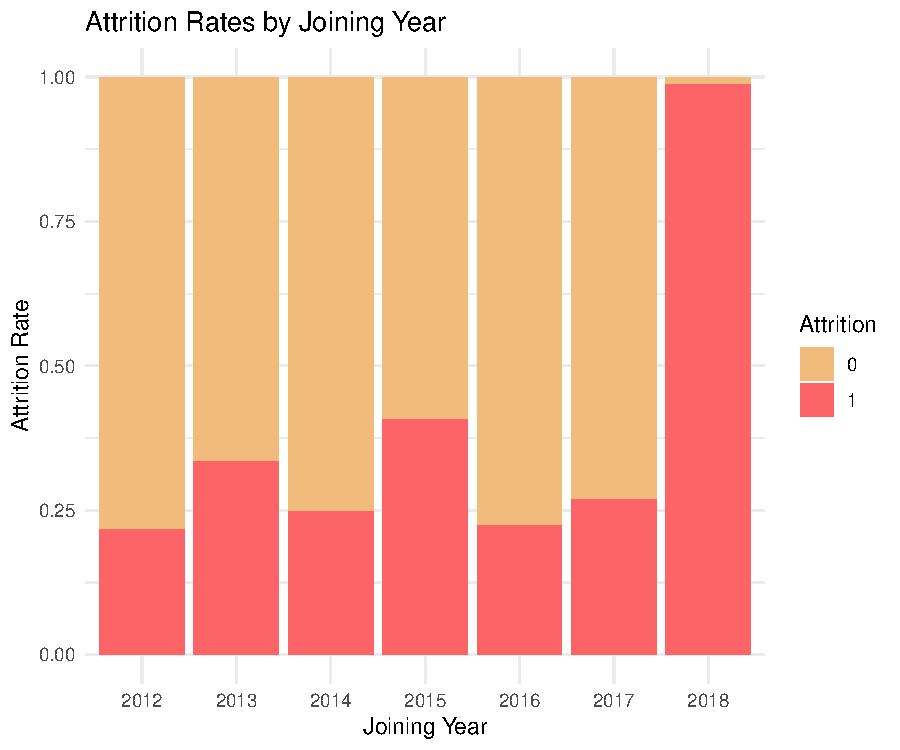
\includegraphics{Final_project_files/figure-latex/unnamed-chunk-4-2.pdf}

\hypertarget{feature-and-target-engineering}{%
\section*{Feature and Target
Engineering}\label{feature-and-target-engineering}}
\addcontentsline{toc}{section}{Feature and Target Engineering}

Since my predictor variable (Leave or Not) is binary, there is no need
for target engineering.

Regarding feature engineering, most of the features are categorical.
Gender and whether a person benched or not (removed themselves from
projects in the lst month) are transformed into dummies. Joining year is
one-hot encoded, resulting in binary variables for each of the 5 joining
years.

Education is label encoded as it can be ordered (Bachelors being the
lowest level of education, Master's one higher and PHD being the highest
level of education). Payment Tier and experience in the current domain
were already label encoded and thus do not require further engineering.

Since age is numeric and random forests are able to handle both numeric
and categorical variables, it is not altered.

\hypertarget{logistic-regression}{%
\section*{Logistic Regression}\label{logistic-regression}}
\addcontentsline{toc}{section}{Logistic Regression}

\begin{table}[H]
\centering
\begin{tabular}{rrrrrrrr}
  \hline
 & Min. & 1st Qu. & Median & Mean & 3rd Qu. & Max. & NA's \\ 
  \hline
1 & 0.63 & 0.64 & 0.65 & 0.64 & 0.66 & 0.66 & 0.00 \\ 
  2 & 0.60 & 0.62 & 0.63 & 0.63 & 0.65 & 0.66 & 0.00 \\ 
  3 & 0.70 & 0.72 & 0.74 & 0.74 & 0.75 & 0.76 & 0.00 \\ 
   \hline
\end{tabular}
\caption{Short Table Example \label{tab1}} 
\end{table}

From the logistic regression, model accuracy ranges from 70 and 76
percent for the full model. The weakest model is model 1, which
regresses attrition on education, has an accuracy rate between 63 and 66
percent.

In terms of the most important features, gender and the joining year of
2017 are the most important predictive features. Most of the other
variables do carry some level of importance, therefore the model is not
overly reliant on gender and joining year.

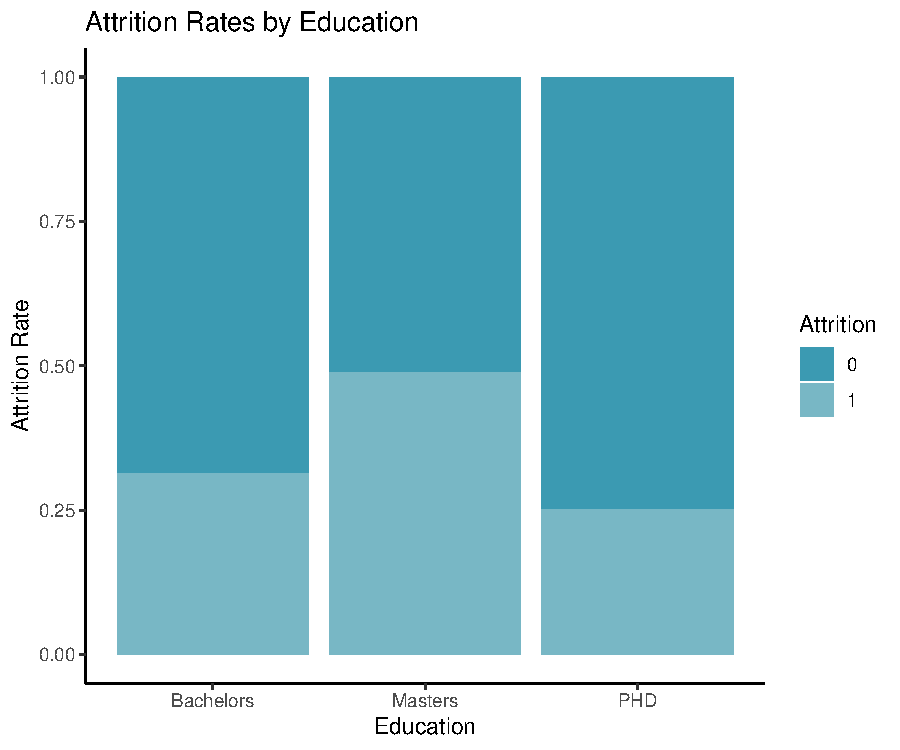
\includegraphics{Final_project_files/figure-latex/unnamed-chunk-7-1.pdf}

\begin{table}[H]
\centering
\begin{tabular}{rlrrrr}
  \hline
 & term & estimate & std.error & statistic & p.value \\ 
  \hline
1 & (Intercept) & 1.86 & 0.39 & 4.79 & 0.00 \\ 
  2 & Age & -0.02 & 0.01 & -2.73 & 0.01 \\ 
  3 & male1 & -0.81 & 0.09 & -9.48 & 0.00 \\ 
  4 & benched1 & 0.67 & 0.13 & 5.29 & 0.00 \\ 
  5 & ExperienceInCurrentDomain & -0.07 & 0.03 & -2.48 & 0.01 \\ 
  6 & bangalore1 & 0.17 & 0.12 & 1.45 & 0.15 \\ 
  7 & pune1 & 0.99 & 0.12 & 8.38 & 0.00 \\ 
  8 & education & 0.53 & 0.08 & 6.31 & 0.00 \\ 
  9 & PaymentTier & -0.60 & 0.08 & -7.75 & 0.00 \\ 
  10 & Y2014 & -0.97 & 0.13 & -7.56 & 0.00 \\ 
  11 & Y2015 & -0.69 & 0.12 & -5.63 & 0.00 \\ 
  12 & Y2016 & -1.23 & 0.15 & -8.23 & 0.00 \\ 
  13 & Y2017 & -1.30 & 0.12 & -11.16 & 0.00 \\ 
   \hline
\end{tabular}
\caption{Logistic Regression Results \label{tab1}} 
\end{table}

\hypertarget{knn}{%
\section*{KNN}\label{knn}}
\addcontentsline{toc}{section}{KNN}

looking at a K-Nearest Neighbours approach, a grid-search is conducted
to find the optimal level of K. The accuracy metric is used, given that
is an appropriate metric for a classification problem. The grid search
looks for the optimal level of K between 2 and 25. The model selects k
=3 as the optimal value. The accuracy rate for k=3 is 78.3\%.

For the testing data, the model's accuracy is slightly lower at 77\%.

\begin{verbatim}
## [1] 0.7743553
\end{verbatim}

\hypertarget{random-forests}{%
\section*{Random Forests}\label{random-forests}}
\addcontentsline{toc}{section}{Random Forests}

Random forests are powerful out-of the box algorithms that generally
have very good predictive accuracy (). The come with the benefits of
decision trees and bagging but greatly reduce instability and
between-tree correlation.

\hypertarget{decision-tree}{%
\subsection*{Decision tree}\label{decision-tree}}
\addcontentsline{toc}{subsection}{Decision tree}

Following the general rule-of-thumb, there is a 70:30 split among the
training and testing data.

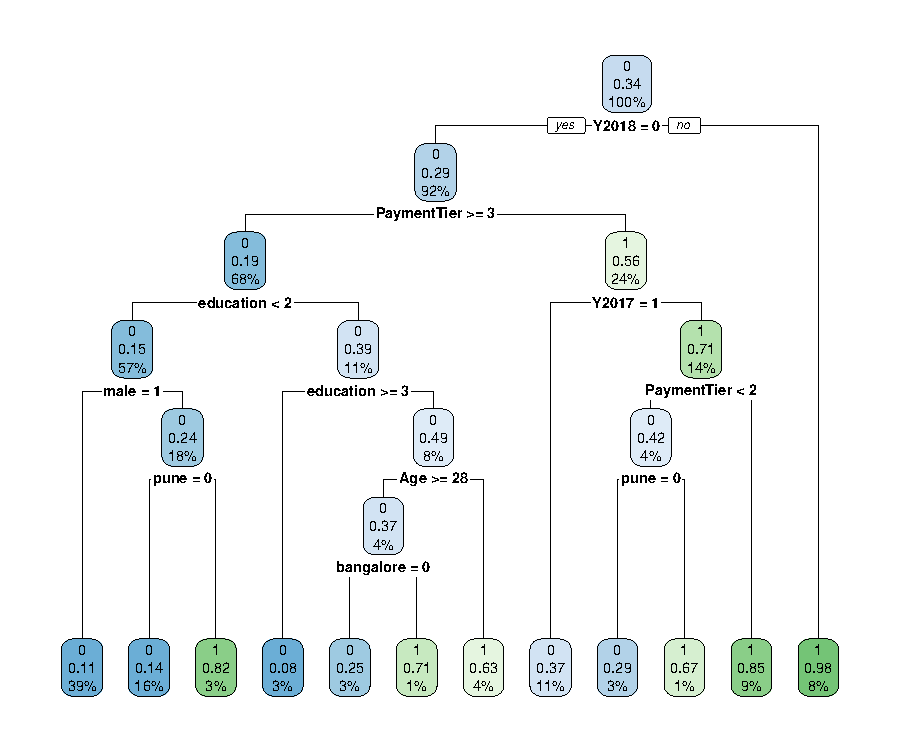
\includegraphics{Final_project_files/figure-latex/unnamed-chunk-8-1.pdf}

\#ranger - model\$confusionmatrix

\begin{verbatim}
## Accuracy: 82.80802 %
\end{verbatim}

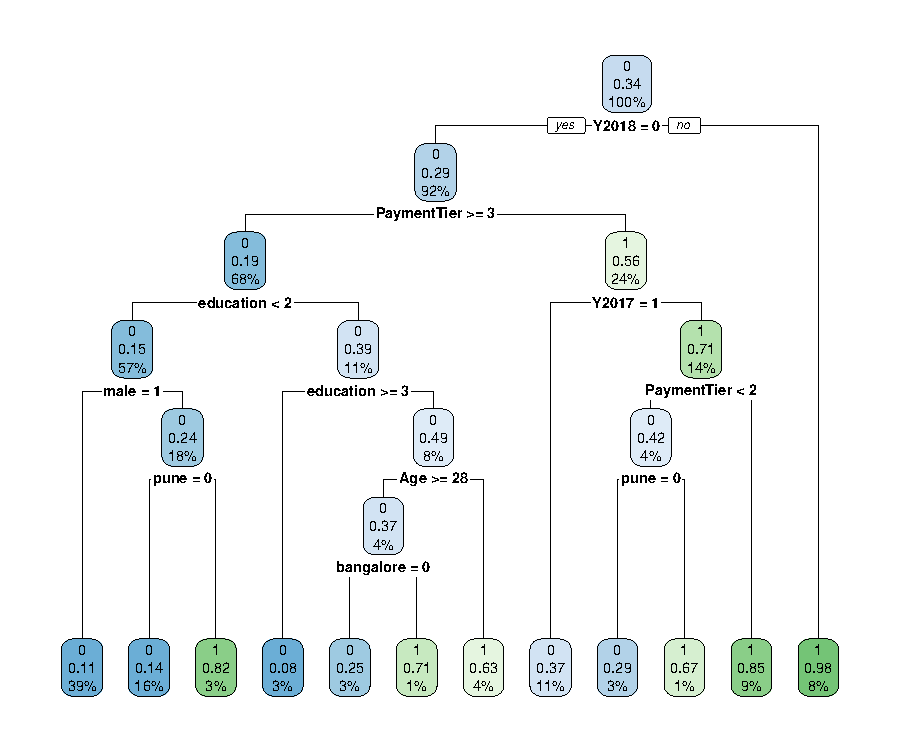
\includegraphics{Final_project_files/figure-latex/unnamed-chunk-9-1.pdf}

The results from the baseline random forest are presented below. Random
Forests help to reduce tree correlation. It does so by using
split-variable randomisation. In the baseline model, number of trees are
set to 500 by default. It is possible to alter the m(try) parameter, but
currently it is set to the square root of the number of parameters,
given that this standard when doing a classification problem.

\begin{verbatim}
## [1] 0.3898466
\end{verbatim}

\begin{table}[H]
\centering
\begin{tabular}{rlr}
  \hline
 & Metric & Value \\ 
  \hline
1 & Accuracy & 0.85 \\ 
  2 & F1 Score & 0.73 \\ 
  3 & Recall & 0.62 \\ 
  4 & Precision & 0.90 \\ 
  5 & AUC ROC & 0.79 \\ 
   \hline
\end{tabular}
\caption{Metrics for Baseline Random Forest \label{tab1}} 
\end{table}

Comparing the training and testing error, the test error (15.1\%) is
slightly higher than the training error (11.8\%). This may indicate that
there is some level of overfitting, given that the training data
performs better, however it does not appear to be substantial. The
model's performance is still reasonably good.

To continue to examine the bias-variance tradeoff, the learning curve is
plotted. At small sample sizes, it can be seen that the test accuracy is
much lower than the training dataset. The high accuracy for the training
set at lower sample sizes indicates overfitting. Once the sample size
reaches over 2000, the accuracy between the training and the testing set
begin to converge, reducing the bias-variance tradeoff.

\begin{table}[H]
\centering
\begin{tabular}{rlr}
  \hline
 & Metric & Value \\ 
  \hline
1 & Training Accuracy & 0.88 \\ 
  2 & Test Accuracy & 0.84 \\ 
  3 & Training Error & 0.12 \\ 
  4 & Test Error & 0.16 \\ 
   \hline
\end{tabular}
\caption{More Metrics for Baseline Random Forest \label{tab1}} 
\end{table}

There are several hyper-parameters to consider in this model, including
the number of trees, the number of features to consider at a given
split, the complexity of each tree, the sampling scheme, and the
splitting rule to use during tree construction.

The first parameter I adjust is the number of trees. If I have 15
variables, I will make 150 trees. The default above was 500 trees.

Adjusting the number of trees down from 500 to 150 increases the
accuracy of the model, but marginally. Accuracy increased from 84.81\%
to 84.96\%.

Following the baseline random forest model, a grid search is conducted
over a range of hyperparameters in an attempt to select the optimal
model.

The default sampling scheme for a random forest is one with replacement.

Sample size influences how many observations are drawn for the training
of each tree. Decreasing the sample size leads to more diverse trees and
less between-tree correlation, which has a positive effect on predictive
accuracy. Having a few features that

Having many categorical features with varying number of levels, such as
experience or education in this case, or unbalanced categories, then
sampling with replacement can lead to biased results. Sampling without
replacement can thus lead to a less biased use of all the levels across
the trees in the random forest.

I included the number of trees in the search. As a rule of thumb, the
number of trees is 100, 150 and 250 were selected as possibilities.

The best model selected is one with m(try) set to 4, a number of trees
as 250, a node size of 1, sample without replacement, and a sample
fraction of 0.63.

\begin{verbatim}
## [1] 0.3741739
\end{verbatim}

\begin{verbatim}
## [1] 0.8495702
\end{verbatim}

\begin{verbatim}
## [1] 0.875
\end{verbatim}

\begin{verbatim}
## [1] 0.65625
\end{verbatim}

\begin{verbatim}
## [1] 0.75
\end{verbatim}

\begin{verbatim}
## Area under the curve: 0.7914
\end{verbatim}

\begin{table}[H]
\centering
\begin{tabular}{rlr}
  \hline
 & Metric & Value \\ 
  \hline
1 & Accuracy & 0.85 \\ 
  2 & F1 Score & 0.75 \\ 
  3 & Recall & 0.66 \\ 
  4 & Precision & 0.88 \\ 
  5 & AUC ROC & 0.79 \\ 
   \hline
\end{tabular}
\caption{Metrics for Tuned Random Forest \label{tab1}} 
\end{table}

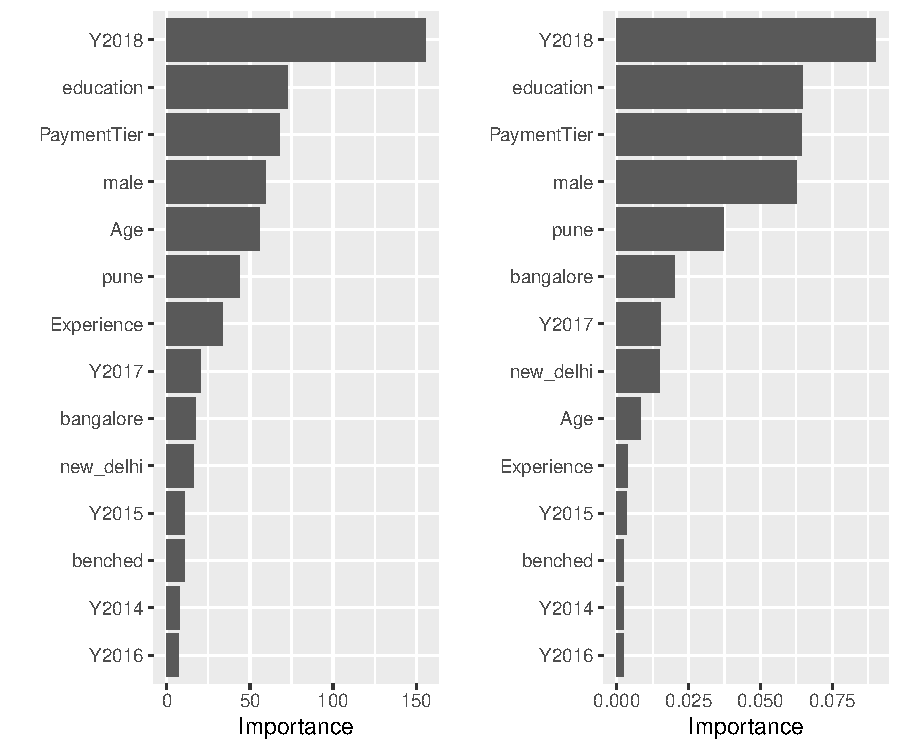
\includegraphics{Final_project_files/figure-latex/unnamed-chunk-13-1.pdf}

\hypertarget{results}{%
\section{Results}\label{results}}

Tables can be included as follows. Use the \emph{xtable} (or kable)
package for tables. Table placement = H implies Latex tries to place the
table Here, and not on a new page (there are, however, very many ways to
skin this cat. Luckily there are many forums online!).

To reference calculations \textbf{in text}, \emph{do this:} From table
\ref{tab1} we see the average value of mpg is 20.98.

Including tables that span across pages, use the following (note that I
add below the table: ``continue on the next page'\,'). This is a neat
way of splitting your table across a page.

Use the following default settings to build your own possibly long
tables. Note that the following will fit on one page if it can, but
cleanly spreads over multiple pages:

\begingroup\fontsize{12pt}{13pt}\selectfont
\begin{longtable}{rrrrrrrrrrr}
\caption{Long Table Example} \\ 
  \toprule
mpg & cyl & disp & hp & drat & wt & qsec & vs & am & gear & carb \\ 
  \hline 
\endhead 
\hline 
{\footnotesize Continued on next page} 
\endfoot 
\endlastfoot 
 \midrule
21.00 & 6.00 & 160.00 & 110.00 & 3.90 & 2.62 & 16.46 & 0.00 & 1.00 & 4.00 & 4.00 \\ 
  21.00 & 6.00 & 160.00 & 110.00 & 3.90 & 2.88 & 17.02 & 0.00 & 1.00 & 4.00 & 4.00 \\ 
  22.80 & 4.00 & 108.00 & 93.00 & 3.85 & 2.32 & 18.61 & 1.00 & 1.00 & 4.00 & 1.00 \\ 
  21.40 & 6.00 & 258.00 & 110.00 & 3.08 & 3.21 & 19.44 & 1.00 & 0.00 & 3.00 & 1.00 \\ 
  18.70 & 8.00 & 360.00 & 175.00 & 3.15 & 3.44 & 17.02 & 0.00 & 0.00 & 3.00 & 2.00 \\ 
  18.10 & 6.00 & 225.00 & 105.00 & 2.76 & 3.46 & 20.22 & 1.00 & 0.00 & 3.00 & 1.00 \\ 
  14.30 & 8.00 & 360.00 & 245.00 & 3.21 & 3.57 & 15.84 & 0.00 & 0.00 & 3.00 & 4.00 \\ 
  24.40 & 4.00 & 146.70 & 62.00 & 3.69 & 3.19 & 20.00 & 1.00 & 0.00 & 4.00 & 2.00 \\ 
  22.80 & 4.00 & 140.80 & 95.00 & 3.92 & 3.15 & 22.90 & 1.00 & 0.00 & 4.00 & 2.00 \\ 
  19.20 & 6.00 & 167.60 & 123.00 & 3.92 & 3.44 & 18.30 & 1.00 & 0.00 & 4.00 & 4.00 \\ 
  17.80 & 6.00 & 167.60 & 123.00 & 3.92 & 3.44 & 18.90 & 1.00 & 0.00 & 4.00 & 4.00 \\ 
  16.40 & 8.00 & 275.80 & 180.00 & 3.07 & 4.07 & 17.40 & 0.00 & 0.00 & 3.00 & 3.00 \\ 
  17.30 & 8.00 & 275.80 & 180.00 & 3.07 & 3.73 & 17.60 & 0.00 & 0.00 & 3.00 & 3.00 \\ 
  15.20 & 8.00 & 275.80 & 180.00 & 3.07 & 3.78 & 18.00 & 0.00 & 0.00 & 3.00 & 3.00 \\ 
  10.40 & 8.00 & 472.00 & 205.00 & 2.93 & 5.25 & 17.98 & 0.00 & 0.00 & 3.00 & 4.00 \\ 
  10.40 & 8.00 & 460.00 & 215.00 & 3.00 & 5.42 & 17.82 & 0.00 & 0.00 & 3.00 & 4.00 \\ 
  14.70 & 8.00 & 440.00 & 230.00 & 3.23 & 5.34 & 17.42 & 0.00 & 0.00 & 3.00 & 4.00 \\ 
  32.40 & 4.00 & 78.70 & 66.00 & 4.08 & 2.20 & 19.47 & 1.00 & 1.00 & 4.00 & 1.00 \\ 
  30.40 & 4.00 & 75.70 & 52.00 & 4.93 & 1.61 & 18.52 & 1.00 & 1.00 & 4.00 & 2.00 \\ 
  33.90 & 4.00 & 71.10 & 65.00 & 4.22 & 1.83 & 19.90 & 1.00 & 1.00 & 4.00 & 1.00 \\ 
  21.50 & 4.00 & 120.10 & 97.00 & 3.70 & 2.46 & 20.01 & 1.00 & 0.00 & 3.00 & 1.00 \\ 
  15.50 & 8.00 & 318.00 & 150.00 & 2.76 & 3.52 & 16.87 & 0.00 & 0.00 & 3.00 & 2.00 \\ 
  15.20 & 8.00 & 304.00 & 150.00 & 3.15 & 3.44 & 17.30 & 0.00 & 0.00 & 3.00 & 2.00 \\ 
  13.30 & 8.00 & 350.00 & 245.00 & 3.73 & 3.84 & 15.41 & 0.00 & 0.00 & 3.00 & 4.00 \\ 
  19.20 & 8.00 & 400.00 & 175.00 & 3.08 & 3.85 & 17.05 & 0.00 & 0.00 & 3.00 & 2.00 \\ 
  27.30 & 4.00 & 79.00 & 66.00 & 4.08 & 1.94 & 18.90 & 1.00 & 1.00 & 4.00 & 1.00 \\ 
  26.00 & 4.00 & 120.30 & 91.00 & 4.43 & 2.14 & 16.70 & 0.00 & 1.00 & 5.00 & 2.00 \\ 
  30.40 & 4.00 & 95.10 & 113.00 & 3.77 & 1.51 & 16.90 & 1.00 & 1.00 & 5.00 & 2.00 \\ 
  15.80 & 8.00 & 351.00 & 264.00 & 4.22 & 3.17 & 14.50 & 0.00 & 1.00 & 5.00 & 4.00 \\ 
  19.70 & 6.00 & 145.00 & 175.00 & 3.62 & 2.77 & 15.50 & 0.00 & 1.00 & 5.00 & 6.00 \\ 
  15.00 & 8.00 & 301.00 & 335.00 & 3.54 & 3.57 & 14.60 & 0.00 & 1.00 & 5.00 & 8.00 \\ 
  21.40 & 4.00 & 121.00 & 109.00 & 4.11 & 2.78 & 18.60 & 1.00 & 1.00 & 4.00 & 2.00 \\ 
   \bottomrule
\end{longtable}
\endgroup

\hfill

\hypertarget{huxtable}{%
\subsection{Huxtable}\label{huxtable}}

Huxtable is a very nice package for making working with tables between
Rmarkdown and Tex easier.

This cost some adjustment to the Tex templates to make it work, but it
now works nicely.

See documentation for this package
\href{https://hughjonesd.github.io/huxtable/huxtable.html}{here}. A
particularly nice addition of this package is for making the printing of
regression results a joy (see
\href{https://hughjonesd.github.io/huxtable/huxtable.html\#creating-a-regression-table}{here}).
Here follows an example:

If you are eager to use huxtable, comment out the Huxtable table in the
Rmd template, and uncomment the colortbl package in your Rmd's root.

Note that I do not include this in the ordinary template, as some latex
users have complained it breaks when they build their Rmds (especially
those using tidytex - I don't have this problem as I have the full
Miktex installed on mine). Up to you, but I strongly recommend
installing the package manually and using huxtable. To make this work,
uncomment the \emph{Adding additional latex packages} part in yaml at
the top of the Rmd file. Then comment out the huxtable example in the
template below this line. Reknit, and enjoy.

 
  \providecommand{\huxb}[2]{\arrayrulecolor[RGB]{#1}\global\arrayrulewidth=#2pt}
  \providecommand{\huxvb}[2]{\color[RGB]{#1}\vrule width #2pt}
  \providecommand{\huxtpad}[1]{\rule{0pt}{#1}}
  \providecommand{\huxbpad}[1]{\rule[-#1]{0pt}{#1}}

\begin{table}[ht]
\begin{centerbox}
\begin{threeparttable}
\captionsetup{justification=centering,singlelinecheck=off}
\caption{Regression Output}
 \label{Reg01}
\setlength{\tabcolsep}{0pt}
\begin{tabular}{l l l l}


\hhline{>{\huxb{0, 0, 0}{0.8}}->{\huxb{0, 0, 0}{0.8}}->{\huxb{0, 0, 0}{0.8}}->{\huxb{0, 0, 0}{0.8}}-}
\arrayrulecolor{black}

\multicolumn{1}{!{\huxvb{0, 0, 0}{0}}c!{\huxvb{0, 0, 0}{0}}}{\huxtpad{6pt + 1em}\centering \hspace{6pt} {\fontsize{12pt}{14.4pt}\selectfont } \hspace{6pt}\huxbpad{6pt}} &
\multicolumn{1}{c!{\huxvb{0, 0, 0}{0}}}{\huxtpad{6pt + 1em}\centering \hspace{6pt} {\fontsize{12pt}{14.4pt}\selectfont Reg1} \hspace{6pt}\huxbpad{6pt}} &
\multicolumn{1}{c!{\huxvb{0, 0, 0}{0}}}{\huxtpad{6pt + 1em}\centering \hspace{6pt} {\fontsize{12pt}{14.4pt}\selectfont Reg2} \hspace{6pt}\huxbpad{6pt}} &
\multicolumn{1}{c!{\huxvb{0, 0, 0}{0}}}{\huxtpad{6pt + 1em}\centering \hspace{6pt} {\fontsize{12pt}{14.4pt}\selectfont Reg3} \hspace{6pt}\huxbpad{6pt}} \tabularnewline[-0.5pt]


\hhline{>{\huxb{255, 255, 255}{0.4}}->{\huxb{0, 0, 0}{0.4}}->{\huxb{0, 0, 0}{0.4}}->{\huxb{0, 0, 0}{0.4}}-}
\arrayrulecolor{black}

\multicolumn{1}{!{\huxvb{0, 0, 0}{0}}l!{\huxvb{0, 0, 0}{0}}}{\huxtpad{6pt + 1em}\raggedright \hspace{6pt} {\fontsize{12pt}{14.4pt}\selectfont (Intercept)} \hspace{6pt}\huxbpad{6pt}} &
\multicolumn{1}{r!{\huxvb{0, 0, 0}{0}}}{\huxtpad{6pt + 1em}\raggedleft \hspace{6pt} {\fontsize{12pt}{14.4pt}\selectfont -2256.361 ***} \hspace{6pt}\huxbpad{6pt}} &
\multicolumn{1}{r!{\huxvb{0, 0, 0}{0}}}{\huxtpad{6pt + 1em}\raggedleft \hspace{6pt} {\fontsize{12pt}{14.4pt}\selectfont 5763.668 ***} \hspace{6pt}\huxbpad{6pt}} &
\multicolumn{1}{r!{\huxvb{0, 0, 0}{0}}}{\huxtpad{6pt + 1em}\raggedleft \hspace{6pt} {\fontsize{12pt}{14.4pt}\selectfont 4045.333 ***} \hspace{6pt}\huxbpad{6pt}} \tabularnewline[-0.5pt]


\hhline{}
\arrayrulecolor{black}

\multicolumn{1}{!{\huxvb{0, 0, 0}{0}}l!{\huxvb{0, 0, 0}{0}}}{\huxtpad{6pt + 1em}\raggedright \hspace{6pt} {\fontsize{12pt}{14.4pt}\selectfont } \hspace{6pt}\huxbpad{6pt}} &
\multicolumn{1}{r!{\huxvb{0, 0, 0}{0}}}{\huxtpad{6pt + 1em}\raggedleft \hspace{6pt} {\fontsize{12pt}{14.4pt}\selectfont (13.055)\hphantom{0}\hphantom{0}\hphantom{0}} \hspace{6pt}\huxbpad{6pt}} &
\multicolumn{1}{r!{\huxvb{0, 0, 0}{0}}}{\huxtpad{6pt + 1em}\raggedleft \hspace{6pt} {\fontsize{12pt}{14.4pt}\selectfont (740.556)\hphantom{0}\hphantom{0}\hphantom{0}} \hspace{6pt}\huxbpad{6pt}} &
\multicolumn{1}{r!{\huxvb{0, 0, 0}{0}}}{\huxtpad{6pt + 1em}\raggedleft \hspace{6pt} {\fontsize{12pt}{14.4pt}\selectfont (286.205)\hphantom{0}\hphantom{0}\hphantom{0}} \hspace{6pt}\huxbpad{6pt}} \tabularnewline[-0.5pt]


\hhline{}
\arrayrulecolor{black}

\multicolumn{1}{!{\huxvb{0, 0, 0}{0}}l!{\huxvb{0, 0, 0}{0}}}{\huxtpad{6pt + 1em}\raggedright \hspace{6pt} {\fontsize{12pt}{14.4pt}\selectfont carat} \hspace{6pt}\huxbpad{6pt}} &
\multicolumn{1}{r!{\huxvb{0, 0, 0}{0}}}{\huxtpad{6pt + 1em}\raggedleft \hspace{6pt} {\fontsize{12pt}{14.4pt}\selectfont 7756.426 ***} \hspace{6pt}\huxbpad{6pt}} &
\multicolumn{1}{r!{\huxvb{0, 0, 0}{0}}}{\huxtpad{6pt + 1em}\raggedleft \hspace{6pt} {\fontsize{12pt}{14.4pt}\selectfont \hphantom{0}\hphantom{0}\hphantom{0}\hphantom{0}\hphantom{0}\hphantom{0}\hphantom{0}\hphantom{0}} \hspace{6pt}\huxbpad{6pt}} &
\multicolumn{1}{r!{\huxvb{0, 0, 0}{0}}}{\huxtpad{6pt + 1em}\raggedleft \hspace{6pt} {\fontsize{12pt}{14.4pt}\selectfont 7765.141 ***} \hspace{6pt}\huxbpad{6pt}} \tabularnewline[-0.5pt]


\hhline{}
\arrayrulecolor{black}

\multicolumn{1}{!{\huxvb{0, 0, 0}{0}}l!{\huxvb{0, 0, 0}{0}}}{\huxtpad{6pt + 1em}\raggedright \hspace{6pt} {\fontsize{12pt}{14.4pt}\selectfont } \hspace{6pt}\huxbpad{6pt}} &
\multicolumn{1}{r!{\huxvb{0, 0, 0}{0}}}{\huxtpad{6pt + 1em}\raggedleft \hspace{6pt} {\fontsize{12pt}{14.4pt}\selectfont (14.067)\hphantom{0}\hphantom{0}\hphantom{0}} \hspace{6pt}\huxbpad{6pt}} &
\multicolumn{1}{r!{\huxvb{0, 0, 0}{0}}}{\huxtpad{6pt + 1em}\raggedleft \hspace{6pt} {\fontsize{12pt}{14.4pt}\selectfont \hphantom{0}\hphantom{0}\hphantom{0}\hphantom{0}\hphantom{0}\hphantom{0}\hphantom{0}\hphantom{0}} \hspace{6pt}\huxbpad{6pt}} &
\multicolumn{1}{r!{\huxvb{0, 0, 0}{0}}}{\huxtpad{6pt + 1em}\raggedleft \hspace{6pt} {\fontsize{12pt}{14.4pt}\selectfont (14.009)\hphantom{0}\hphantom{0}\hphantom{0}} \hspace{6pt}\huxbpad{6pt}} \tabularnewline[-0.5pt]


\hhline{}
\arrayrulecolor{black}

\multicolumn{1}{!{\huxvb{0, 0, 0}{0}}l!{\huxvb{0, 0, 0}{0}}}{\huxtpad{6pt + 1em}\raggedright \hspace{6pt} {\fontsize{12pt}{14.4pt}\selectfont depth} \hspace{6pt}\huxbpad{6pt}} &
\multicolumn{1}{r!{\huxvb{0, 0, 0}{0}}}{\huxtpad{6pt + 1em}\raggedleft \hspace{6pt} {\fontsize{12pt}{14.4pt}\selectfont \hphantom{0}\hphantom{0}\hphantom{0}\hphantom{0}\hphantom{0}\hphantom{0}\hphantom{0}\hphantom{0}} \hspace{6pt}\huxbpad{6pt}} &
\multicolumn{1}{r!{\huxvb{0, 0, 0}{0}}}{\huxtpad{6pt + 1em}\raggedleft \hspace{6pt} {\fontsize{12pt}{14.4pt}\selectfont -29.650 *\hphantom{0}\hphantom{0}} \hspace{6pt}\huxbpad{6pt}} &
\multicolumn{1}{r!{\huxvb{0, 0, 0}{0}}}{\huxtpad{6pt + 1em}\raggedleft \hspace{6pt} {\fontsize{12pt}{14.4pt}\selectfont -102.165 ***} \hspace{6pt}\huxbpad{6pt}} \tabularnewline[-0.5pt]


\hhline{}
\arrayrulecolor{black}

\multicolumn{1}{!{\huxvb{0, 0, 0}{0}}l!{\huxvb{0, 0, 0}{0}}}{\huxtpad{6pt + 1em}\raggedright \hspace{6pt} {\fontsize{12pt}{14.4pt}\selectfont } \hspace{6pt}\huxbpad{6pt}} &
\multicolumn{1}{r!{\huxvb{0, 0, 0}{0}}}{\huxtpad{6pt + 1em}\raggedleft \hspace{6pt} {\fontsize{12pt}{14.4pt}\selectfont \hphantom{0}\hphantom{0}\hphantom{0}\hphantom{0}\hphantom{0}\hphantom{0}\hphantom{0}\hphantom{0}} \hspace{6pt}\huxbpad{6pt}} &
\multicolumn{1}{r!{\huxvb{0, 0, 0}{0}}}{\huxtpad{6pt + 1em}\raggedleft \hspace{6pt} {\fontsize{12pt}{14.4pt}\selectfont (11.990)\hphantom{0}\hphantom{0}\hphantom{0}} \hspace{6pt}\huxbpad{6pt}} &
\multicolumn{1}{r!{\huxvb{0, 0, 0}{0}}}{\huxtpad{6pt + 1em}\raggedleft \hspace{6pt} {\fontsize{12pt}{14.4pt}\selectfont (4.635)\hphantom{0}\hphantom{0}\hphantom{0}} \hspace{6pt}\huxbpad{6pt}} \tabularnewline[-0.5pt]


\hhline{>{\huxb{255, 255, 255}{0.4}}->{\huxb{0, 0, 0}{0.4}}->{\huxb{0, 0, 0}{0.4}}->{\huxb{0, 0, 0}{0.4}}-}
\arrayrulecolor{black}

\multicolumn{1}{!{\huxvb{0, 0, 0}{0}}l!{\huxvb{0, 0, 0}{0}}}{\huxtpad{6pt + 1em}\raggedright \hspace{6pt} {\fontsize{12pt}{14.4pt}\selectfont N} \hspace{6pt}\huxbpad{6pt}} &
\multicolumn{1}{r!{\huxvb{0, 0, 0}{0}}}{\huxtpad{6pt + 1em}\raggedleft \hspace{6pt} {\fontsize{12pt}{14.4pt}\selectfont 53940\hphantom{0}\hphantom{0}\hphantom{0}\hphantom{0}\hphantom{0}\hphantom{0}\hphantom{0}\hphantom{0}} \hspace{6pt}\huxbpad{6pt}} &
\multicolumn{1}{r!{\huxvb{0, 0, 0}{0}}}{\huxtpad{6pt + 1em}\raggedleft \hspace{6pt} {\fontsize{12pt}{14.4pt}\selectfont 53940\hphantom{0}\hphantom{0}\hphantom{0}\hphantom{0}\hphantom{0}\hphantom{0}\hphantom{0}\hphantom{0}} \hspace{6pt}\huxbpad{6pt}} &
\multicolumn{1}{r!{\huxvb{0, 0, 0}{0}}}{\huxtpad{6pt + 1em}\raggedleft \hspace{6pt} {\fontsize{12pt}{14.4pt}\selectfont 53940\hphantom{0}\hphantom{0}\hphantom{0}\hphantom{0}\hphantom{0}\hphantom{0}\hphantom{0}\hphantom{0}} \hspace{6pt}\huxbpad{6pt}} \tabularnewline[-0.5pt]


\hhline{}
\arrayrulecolor{black}

\multicolumn{1}{!{\huxvb{0, 0, 0}{0}}l!{\huxvb{0, 0, 0}{0}}}{\huxtpad{6pt + 1em}\raggedright \hspace{6pt} {\fontsize{12pt}{14.4pt}\selectfont R2} \hspace{6pt}\huxbpad{6pt}} &
\multicolumn{1}{r!{\huxvb{0, 0, 0}{0}}}{\huxtpad{6pt + 1em}\raggedleft \hspace{6pt} {\fontsize{12pt}{14.4pt}\selectfont 0.849\hphantom{0}\hphantom{0}\hphantom{0}\hphantom{0}} \hspace{6pt}\huxbpad{6pt}} &
\multicolumn{1}{r!{\huxvb{0, 0, 0}{0}}}{\huxtpad{6pt + 1em}\raggedleft \hspace{6pt} {\fontsize{12pt}{14.4pt}\selectfont 0.000\hphantom{0}\hphantom{0}\hphantom{0}\hphantom{0}} \hspace{6pt}\huxbpad{6pt}} &
\multicolumn{1}{r!{\huxvb{0, 0, 0}{0}}}{\huxtpad{6pt + 1em}\raggedleft \hspace{6pt} {\fontsize{12pt}{14.4pt}\selectfont 0.851\hphantom{0}\hphantom{0}\hphantom{0}\hphantom{0}} \hspace{6pt}\huxbpad{6pt}} \tabularnewline[-0.5pt]


\hhline{>{\huxb{0, 0, 0}{0.8}}->{\huxb{0, 0, 0}{0.8}}->{\huxb{0, 0, 0}{0.8}}->{\huxb{0, 0, 0}{0.8}}-}
\arrayrulecolor{black}

\multicolumn{4}{!{\huxvb{0, 0, 0}{0}}l!{\huxvb{0, 0, 0}{0}}}{\huxtpad{6pt + 1em}\raggedright \hspace{6pt} {\fontsize{12pt}{14.4pt}\selectfont  *** p $<$ 0.001;  ** p $<$ 0.01;  * p $<$ 0.05.} \hspace{6pt}\huxbpad{6pt}} \tabularnewline[-0.5pt]


\hhline{}
\arrayrulecolor{black}
\end{tabular}
\end{threeparttable}\par\end{centerbox}

\end{table}
 

FYI - R also recently introduced the gt package, which is worthwhile
exploring too.

\hypertarget{lists}{%
\section{Lists}\label{lists}}

To add lists, simply using the following notation

\begin{itemize}
\item
  This is really simple

  \begin{itemize}
  \tightlist
  \item
    Just note the spaces here - writing in R you have to sometimes be
    pedantic about spaces\ldots{}
  \end{itemize}
\item
  Note that Rmarkdown notation removes the pain of defining
  \LaTeX environments!
\end{itemize}

\hypertarget{conclusion}{%
\section{Conclusion}\label{conclusion}}

I hope you find this template useful. Remember, stackoverflow is your
friend - use it to find answers to questions. Feel free to write me a
mail if you have any questions regarding the use of this package. To
cite this package, simply type citation(``Texevier'') in Rstudio to get
the citation for Katzke (\protect\hyperlink{ref-Texevier}{2017}) (Note
that uncited references in your bibtex file will not be included in
References).

\newpage

\hypertarget{references}{%
\section*{References}\label{references}}
\addcontentsline{toc}{section}{References}

\hypertarget{refs}{}
\begin{CSLReferences}{1}{0}
\leavevmode\vadjust pre{\hypertarget{ref-Texevier}{}}%
Katzke, N.F. 2017. \emph{{Texevier}: {P}ackage to create elsevier
templates for rmarkdown}. Stellenbosch, South Africa: Bureau for
Economic Research.

\end{CSLReferences}

\hypertarget{appendix}{%
\section*{Appendix}\label{appendix}}
\addcontentsline{toc}{section}{Appendix}

\hypertarget{appendix-a}{%
\subsection*{Appendix A}\label{appendix-a}}
\addcontentsline{toc}{subsection}{Appendix A}

Some appendix information here

\hypertarget{appendix-b}{%
\subsection*{Appendix B}\label{appendix-b}}
\addcontentsline{toc}{subsection}{Appendix B}

\bibliography{Tex/ref}





\end{document}
